\documentclass[11pt]{article}
\usepackage[margin=1in]{geometry}
\usepackage{amsmath,amsthm,amssymb}
\usepackage{enumitem, graphicx, float, caption}
\usepackage{amsmath}
\usepackage{bm}
\usepackage{parskip}
\usepackage{lipsum}
\usepackage{tikz}
\usepackage{listings}
\usepackage{xcolor}
\usepackage{float}
\usepackage{subcaption}
\usepackage{graphicx}
\usepackage[utf8]{inputenc}
\usetikzlibrary{arrows.meta}

\definecolor{codegreen}{rgb}{0,0.6,0}
\definecolor{codegray}{rgb}{0.5,0.5,0.5}
\definecolor{codepurple}{rgb}{0.58,0,0.82}
\definecolor{backcolour}{rgb}{0.95,0.95,0.92}

\lstdefinestyle{mystyle}{
    backgroundcolor=\color{backcolour},
    commentstyle=\color{codegreen},
    keywordstyle=\color{magenta},
    numberstyle=\tiny\color{codegray},
    stringstyle=\color{codepurple},
    basicstyle=\ttfamily\tiny,
    breakatwhitespace=false,
    breaklines=true,
    captionpos=b,
    keepspaces=true,
    numbers=left,
    numbersep=5pt,
    showspaces=false,
    showstringspaces=false,
    showtabs=false,
    tabsize=2
}

\lstset{xleftmargin=.020\textwidth, xrightmargin=.020\textwidth}

\setcounter{MaxMatrixCols}{26}
\setlength\parindent{0pt}
\counterwithin{equation}{enumi}


\begin{document}
    \noindent Nathan Burwig \\
    Math 87 HW 10 \\
    Due 12/9/2022
    
    \hrulefill
    
    \section{Visualizing Lotka-Volterra}
    \begin{enumerate}
        \item We can attempt to intuitively understand the following
            equations...
            \begin{align*}
                \frac{\partial r}{\partial t} &= r(\alpha - \beta f) \\
                \frac{\partial f}{\partial t} &= f(\delta r - \gamma)
            \end{align*}
            We consider f to be the population of the foxes, and r to be the
            population of the rabbits. Then $\frac{\partial r}{\partial t}$ is
            the rate of change of the rabbit population and same for the foxes.

            We can see that the rabit population depends linearly on the
            current rabit population times some constant $\alpha$. This makes
            sense, as we would expect the rabbit population to increase with
            the total rabbit population due to breeding.

            It also has a negative term associated with the number of foxes as
            well as the number of rabbits. This is due to the foxes eating the
            rabbits. 

            Similarly we have a positive term dependent on the number of foxes
            and rabbits in the fox population equation. This is because the
            more rabbits the foxes eat, the higher their expected population
            growth. There is equally a negative population term associated with
            the starvation of a fox.

            Thus we can see why this model might be reasonable for a small
            scale idealized system.

        \item We want to write a function in python that handles the above
            equation and returns the result in an array (vector) or ideally a
            numpy array. I wrote the following code.

            \begin{lstlisting}[style=mystyle, linewidth=0.94\linewidth, 
                                language=Python, gobble=8, caption=Gradient Function]
                # initial conditions
                params1  = [1., 0.1, 1.5, .75]
                params2  = np.random.rand(4)
                pops     = [10, 5]
                dt       = 1000
                minT     = 0
                maxT     = 15
                
                a,b,c,d      = params1
                t            = np.linspace(minT, maxT, dt)
                
                ## we have to create our function rather specifically so we can use the odeint function
                ## we have a dummy varibale t, and then all our intial conditions
                def gradient(pop_vec, t):
                    R = pop_vec[0]
                    F = pop_vec[1]
                    return np.array([R * (a - b*F), 
                                     F * (d*R - c)])
            \end{lstlisting}

            I decided to keep the initial conditions as global constants as I
            continue using them later in the project. Passing them into the
            function then is of little use, and complicates the \texttt{scipy}
            integration step by required an extra \texttt{args} tuple.

            When we evaluate the gradient for a given $(r,f)$ value pair we are
            characterizing the rate of change of our state space. In general
            the gradient characterizes the direction of the rate of fastest
            increase. In this case, though, it is characterizing the rate of
            our population change for both foxes and rabbits.

        \item Integrating the equations from some starting time t to a later
            time t'. The values of these integrals for either function would
            likely indicate the total population size at a given time step
            $\Delta t$. I believe that will be more apparent when we do the
            next part of the problem.

        \item We can go ahead and execute and plot the integrals we used above
            utilizing \texttt{scipy.integrate.odeint}. The code I wrote looks
            like the following.

            \begin{lstlisting}[style=mystyle, linewidth=0.94\linewidth, 
                                language=Python, gobble=8, caption=scipy integrate]
                sol = integrate.odeint(gradient, pops, t)
                rabbits, foxes = sol.T
            \end{lstlisting}

            This was pretty straightforward, and you can find the \texttt{pops}
            array in my initial conditions in Listing 1. I take the transpose
            here as, otherwise, the data isn't easily plottable in 2D. For the
            initial conditions I gave above (ie params1) we get a nice periodic
            plot. 
            \begin{center}
                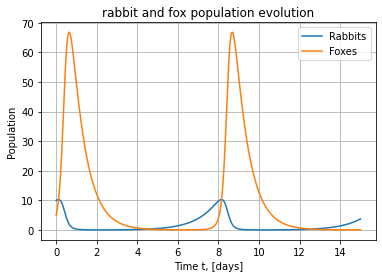
\includegraphics[width=.5\linewidth]{output.png}
            \end{center}
            However, if we utilize some alternate initial conditions (params2
            which) we get (more often than not) something that is not periodic 
            within 15 days. 

            \begin{minipage}[t]{0.5\linewidth}
                \begin{center}
                    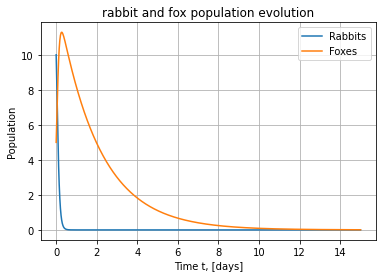
\includegraphics[width=.9\linewidth]{output1.png}
                \end{center}
            \end{minipage}%
            \begin{minipage}[t]{0.5\linewidth}
                \begin{center}
                    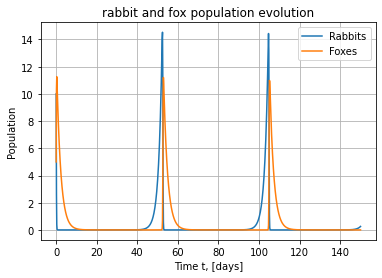
\includegraphics[width=.9\linewidth]{output3.png}
                \end{center}
            \end{minipage}

            Above I've put the associated integral plots, one showing a range
            of 15 and the other of 150 to show that, almost no matter what,
            this is a periodic system. 

        \item Full disclosure, I had some trouble with this section because I
            was not familiar with \\ \texttt{matplotlib.pyplot.quiver} or
            \texttt{numpy.meshgrid}. After much fiddling around, though, I was
            able to produce the following.

            \begin{minipage}[t]{0.5\linewidth}
                \begin{center}
                    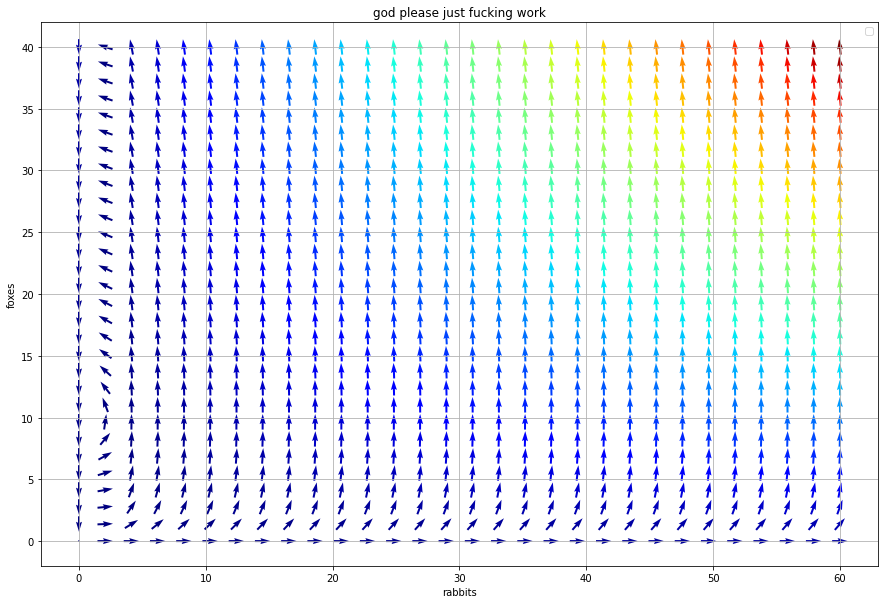
\includegraphics[width=.9\linewidth]{vec1.png}
                \end{center}
            \end{minipage}%
            \begin{minipage}[t]{0.5\linewidth}
                \begin{center}
                    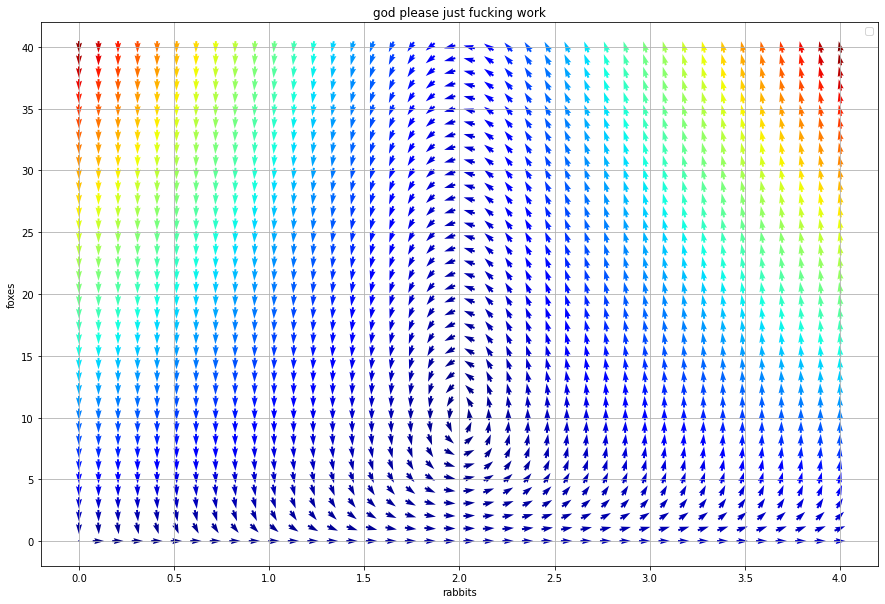
\includegraphics[width=.9\linewidth]{vec2.png}
                \end{center}
            \end{minipage}

        \item The two images above show my vector field graphs. On the right is
            the plot I was able to produce using the given inputs. I noticed,
            though, that there wasn't anything that would seemingly indicate a
            periodic nature in the vector field (loops). In fact, the vector
            field was surprisingly barren.

            I decided to try and crank up the resolution a bit, so I set my
            interpolation to 40 and, noticing the small swirll towards the
            origin, I cut my rabbits axis down to just 4. What results is the
            sort of swirling pattern I was expecting. Note, this is all for
            params1, params2 is not shown here.

            But yes, in general it is good to see the swirls indicating that
            the "stable" states are periodic (as seen in part 4) to some degree depending on the
            inital population conditions.

        \item There are a few unrealistic assumptions made by the
            Lotka-Volterra model. One that I thought about is how it seemingly
            has some issues being solved analytically as you add more
            predators. If you were to try and model a full blown ecological
            system, you would have $n$ coupled differential equations which I
            imagine trying to solve analytically would be a pain.

            As far as assumptions go, though, it assumes constant rates for
            hunting and death in different populations. It also assumes that,
            if necessary, a single predator could cosume rabbits indefinitely
            until dead or that it could consume rabbits every day. It also
            doesn't have any ability (in this formulation at least) to consider
            population caps.

            Overall, the model sacrifices some realism for simplicity, and is
            probably pretty okay for modelling small scale systems, or at the
            very least, fun toy models.

        \item I believe a predator prey model with two predators, one of which
            being a super predator, would look like this...
            \begin{align*}
                \frac{\partial r}{\partial t} &= \alpha r - \beta r f - \psi rh \\
                \frac{\partial f}{\partial t} &= -\gamma f + \delta rf - \omega fh \\
                \frac{\partial h}{\partial t} &= -\lambda h + \phi hr + \eta hf \\
            \end{align*}
            Where I have simply added "interference" terms with the himans in
            the mix. We have two positive terms associated with the human
            population, and one negative, similar to the fox in the previous
            system. We then have negative terms added to the fox and rabbit
            systems to show that humans are hunting both of them.

    \end{enumerate}

\end{document}

